%
% $RCSfile: layers.tex,v $
%
% Copyright (C) 2002-2008. Christian Heller.
%
% Permission is granted to copy, distribute and/or modify this document
% under the terms of the GNU Free Documentation License, Version 1.1 or
% any later version published by the Free Software Foundation; with no
% Invariant Sections, with no Front-Cover Texts and with no Back-Cover
% Texts. A copy of the license is included in the section entitled
% "GNU Free Documentation License".
%
% http://www.cybop.net
% - Cybernetics Oriented Programming -
%
% http://www.resmedicinae.org
% - Information in Medicine -
%
% Version: $Revision: 1.1 $ $Date: 2008-08-19 20:41:07 $ $Author: christian $
% Authors: Christian Heller <christian.heller@tuxtax.de>
%

\subsubsection{Layers}
\label{layers_heading}
\index{Layers Pattern}
\index{Presentation Layer}
\index{Domain Logic Layer}
\index{Business Logic Layer}
\index{Data Source Layer}
\index{ISO OSI Model Layers}
\index{Relaxed Layered System}

The \emph{Layers} pattern \cite{buschmann} is one of the most often used
principles to subdivide a system into logical levels. One variant was shown in
figure \ref{logical_figure}, at the beginning of this chapter. It contained the
three layers \emph{Presentation}, \emph{Domain Logic} and \emph{Data Source}. A
more general illustration can be seen in figure \ref{layers_figure}. It shows a
client using the functionality encapsulated in a layer. That top-most layer
delegates subtasks to lower-level layers which are specialised on solving them.
Another well-known example making use of this pattern is the \emph{ISO OSI}
model as introduced in section \ref{systems_interconnection_heading}.

\begin{figure}[ht]
    \begin{center}
        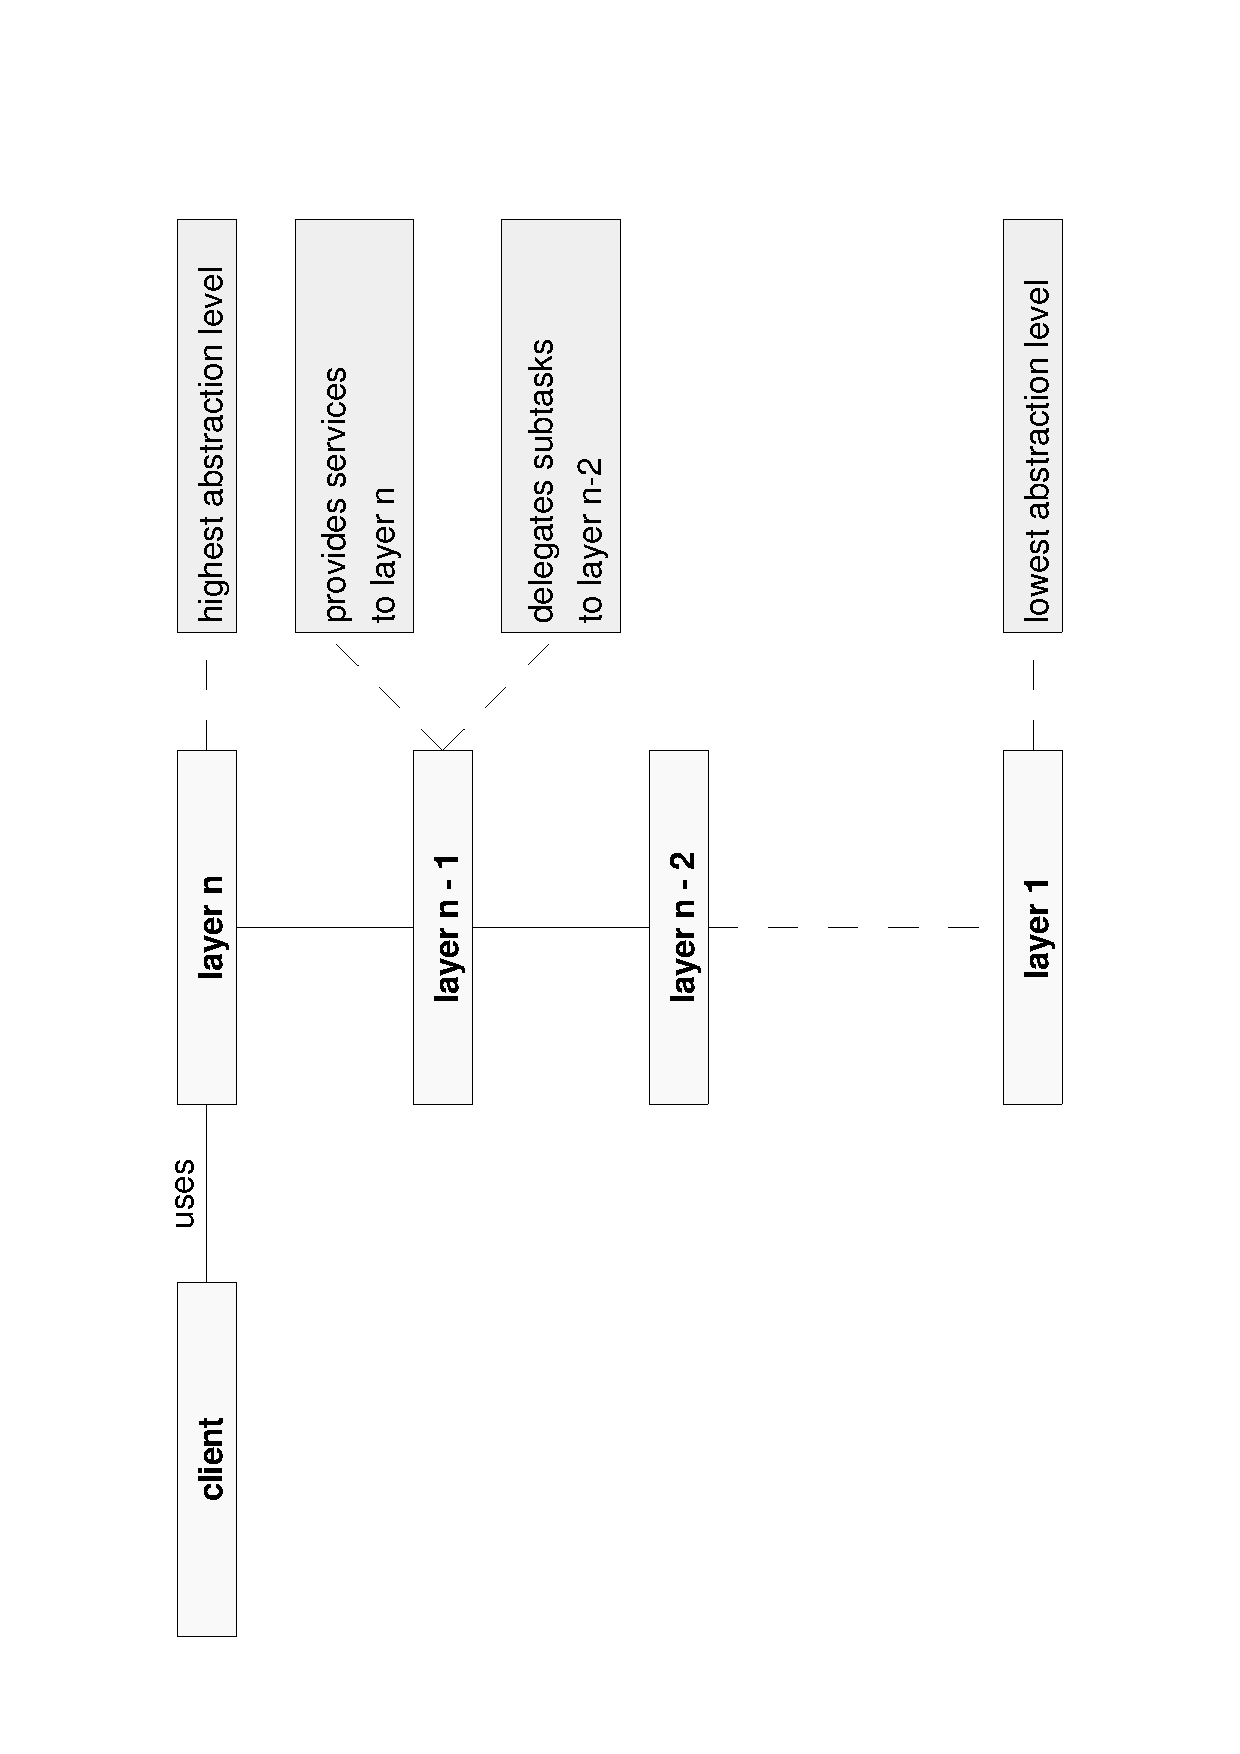
\includegraphics[scale=0.3,angle=-90]{graphic/layers.pdf}
        \caption{Layers Pattern}
        \label{layers_figure}
    \end{center}
\end{figure}

One variant of this pattern, mentioned by Buschmann \cite{buschmann}, is the
\emph{Relaxed-Layered-System}. It permits a layer to not only use the services
of its direct base layer, but also of yet lower-situated layers. The base layer,
in this case, is called \emph{transparent}.

The ontology examples in chapter \ref{knowledge_schema_heading} are organised
according to the \emph{Layers} pattern. Their layers represent levels of
growing granularity.
